\section{Kings: The Tr\'ebuchet and When It Is Exact}\label{sec:kings}

So far a player with no pawn move simply lost. In chess that player would move the king instead, or, with no
king move either, be stalemated, which is a draw. The tr\'ebuchet of Section~\ref{sec:rules} removes
stalemate: a side with no pawn move must move a king, and loses. We now ask when this gives the true chess
result. Our king-and-pawn solver plays real chess, with en passant, stalemate and any of the four
promotions, but no fifty-move rule; an independent reference solver, written from the rules alone, agrees with
it on all $1{,}418{,}480$ positions of its test runs \lab{C2}. Our solver's results below are
\lab{C1} unless a second program or the Lichess tablebase~\cite{LichessTB} confirms them.

\subsection{Two Tr\'ebuchets}

In Fig.~\ref{fig:trebuchet_2025} only the kings can move. White to move must give up a4, since the only square
next to a4 that the king on h5 can move to, h4, is attacked by the a5 pawn across the seam; black to move loses
a5 in the same way. Whoever moves first loses a pawn and then the game, so this is a zero game, and with the
kings played out a real mutual zugzwang that exists only because of the seam \lab{C2}.

Fig.~\ref{fig:trebuchet} shows the same idea on files f to h of the ordinary board; the Lichess tablebase
confirms that it is a mutual zugzwang \lab{C2}. We call this group T and place it beside every ordinary-board
pawn position in this paper.

\begin{figure}[!t]
\centering
\begin{subfigure}{0.32\columnwidth}
\centering
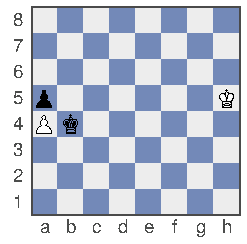
\includegraphics[width=\linewidth]{figures/trebuchet_2025.pdf}
\caption{\pos{W~Kh5~a4 / \mbox{B~Kb4~a5}}}
\label{fig:trebuchet_2025}
\end{subfigure}\hfill
\begin{subfigure}{0.32\columnwidth}
\centering
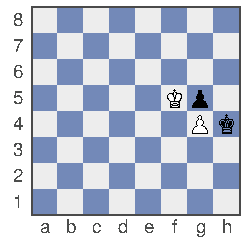
\includegraphics[width=\linewidth]{figures/trebuchet.pdf}
\caption{\pos{W~Kf5~g4 / \mbox{B~Kh4~g5}}}
\label{fig:trebuchet}
\end{subfigure}\hfill
\begin{subfigure}{0.32\columnwidth}
\centering
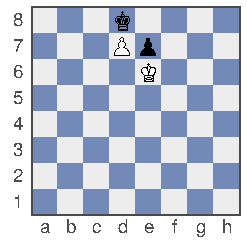
\includegraphics[width=\linewidth]{figures/kinggroup72.pdf}
\caption{\pos{W~Ke6~d7 / \mbox{B~Kd8~e7}}}
\label{fig:kinggroup72}
\end{subfigure}
\caption{King groups: (a) a tr\'ebuchet on the cylinder (files a and h adjacent) and (b) the tr\'ebuchet T
(ordinary board), both real mutual zugzwangs that count as $0$; (c) a king group from the 2025 study (cylinder;
Section~\ref{sec:sums}) that does not count as $0$: it draws with white to move, a zugzwang for black only.}
\label{fig:kings}
\end{figure}

\subsection{When Is the Frozen Tr\'ebuchet Exact?}\label{sec:kings-valid}

A \emph{king group} $Z$ is the two kings and some pawns on a block of files whose neighboring files, the
\emph{buffer}, hold no pawns; a \emph{decisive event} is a move in $Z$ or one creating a passed pawn.

\begin{theorem}[Validity of the convention; \lab{S}]\label{thm:validity}
Let a position consist of pawn components and a king group $Z$ with its buffer, and suppose that before the
first decisive event:
\begin{enumerate}
\item[(V1)] outside $Z$ the legal chess moves are exactly the model's pawn moves, with the same results (en
  passant included); none gives check, nobody is in check, and the side to move has a legal move (one in $Z$
  counts);
\item[(V2)] in chess, the side that gets a passed pawn wins, and a race is won as the race rule says;
\item[(V3)] in chess, every move in $Z$ loses (it is \emph{decisively punished}).
\end{enumerate}
Then the chess result, with either side to move, is the outcome of $W(X)$, the pawn game that ends at the first
passed pawn (Section~\ref{sec:sums-hss}), without draws, where $X$ is the position with $Z$ and its pawns deleted.
\end{theorem}

\begin{proof}[Proof sketch]
By (V3) neither side moves in $Z$ without losing, so until the first decisive event both play the pawn game;
by (V1) the side to move always has a legal move, a pawn move or a move in $Z$; the pawn game is finite, so some
decisive event occurs, and by (V2) and (V3) that event
decides the chess game as it decides $W(X)$.
\end{proof}

\begin{corollary}[\lab{S}]\label{cor:v4}
If also (V4) $X$ is hereditarily sum-safe (Definition~\ref{def:hss}) and satisfies condition (E) of
Theorem~\ref{thm:hss}, and $\BIG$ exceeds the number of moves either side can make, the chess result is
the outcome class of the components' $\pm\BIG$ value.
\end{corollary}

\begin{proof}
By Theorem~\ref{thm:validity} the chess result is the outcome of $W(X)$, and by Theorem~\ref{thm:hss} this is
the outcome of $S(X)$.
\end{proof}

Each condition can fail: a stalemate trap leaves the loser without a move (V1), a passed pawn does not win its
race (V2), a king walks over to the pawns or, in Fig.~\ref{fig:kinggroup72}, white's king moves go unpunished
(V3), and a $+\BIG$ cancels a $-\BIG$ (V4).

A local test for (V3) is the \emph{certificate of horizon $h$} of a move in $Z$: (i) with the pawns outside $Z$
removed, the punisher promotes within $h$ of its own moves after its reply, even if the defender may pass; (ii)
after the reply, with the defender to move and the punisher's king and all pawns in $Z$ removed, no defender
pawn in the context can promote within $h$ of its own moves (its pawns in $Z$ fall under (i)) (the \emph{counter-promotion condition}); (iii) the defender is never stalemated on the forcing
line. It works in the \emph{promotion game}, where the first promotion
wins.

\begin{theorem}[\lab{S}]\label{thm:cert}
In the promotion game, a move in $Z$ with a certificate of horizon $h$ is a loss for its mover, so the
promotion-game analogue of (V3) holds wherever every move in $Z$ has one; for chess, (V3) needs the further
check that a won promotion race is a won game. Clause (ii) cannot be weakened to $h-1$ moves.
\end{theorem}

In chess small margins fail. On the cylinder with seven files and six ranks, Kb4, Pe4 against Ka1, Pa2 with
white to move, the king move Kb4--c5 has a certificate of horizon~1, yet the chess result after it is a draw, and
Kc5--d5 in Kc5, Pe2 against Ka3, Pc4 on the same board has horizon~2, yet White wins \lab{C1}.

For (V2) a local test is known only if king moves also lose \lab{S}: a passed pawn then wins the promotion
game if, besides conditions on checks, stalemates and its own nearby pawns, its path is empty and every enemy
pawn, passed or not, needs a move more to promote. The model looks only at passed pawns: with Pc2, Pd4 against
Pd3 on the $8\times6$ cylinder, black to move, it credits white, yet d3$\times$c2 and c1=Q come first \lab{C1}.

\begin{proposition}[\lab{S}]\label{prop:horizon1}
On boards with at least six ranks, for $h=1$, the counter-promotion condition holds in every chess-legal
context without a passed pawn.
\end{proposition}

\begin{proof}
A pawn that can promote in one move stands on the rank before its last. With six or more ranks it got there by a
single step or a capture, so it cannot be taken en passant, and no enemy pawn can stand ahead of it: it is
already passed.
\end{proof}

\begin{conjecture}[\lab{Conj}]\label{conj:horizon2}
On a board with room for two files beyond the buffer, for every king group whose punishment needs $h\ge2$
moves, some context without a passed pawn leaves a move in the group unpunished.
\end{conjecture}

Real tr\'ebuchets seem to need $h\approx5$--$7$ \lab{Conj}, so we trust their zero only beside slow or locked components.

\subsection{Spare King Moves Are Loopy}

A king that can step back and forth without loss gives its side unlimited waiting moves, a loopy
game~\cite{WinningWays,Siegel2013}: $\textsf{on}=\game{\textsf{on}}{}$ if only white can wait,
$\textsf{off}=-\textsf{on}$ if only black can, and $\textsf{dud}$ if both can. Since $\textsf{on}$ exceeds every number, $\BIG$ included, the $\pm\BIG$ convention fails there, and a
decisive event must instead end the game.

\begin{theorem}[Outcomes with spare moves; \lab{S}]\label{thm:loopy}
Let the components form a short game in which every decisive event ends the game, let a side that can wait pass
at any time, and let every other move in $Z$ lose. If only white can wait, black wins exactly when it can force a decisive
event in its favor against a passing white, and white wins otherwise. If both can wait, a side wins exactly when
it can do so against a passing opponent, and otherwise the game is drawn.
\end{theorem}

\begin{proof}[Proof sketch]
If only white can wait, every play is finite, since black's moves are, so the game is determined, and black
wins exactly when some move of black's wins against every white reply, a pass included. If both can wait, a
winning side never needs to pass, so it wins exactly when it can force a decisive event against passes;
otherwise play can go on forever.
\end{proof}

Beside a spare king move, then, component values matter only through their forcing threats. The kings
alone are already loopy: in normal play (a stalemate loses), every quiet K+P against K placement on the boards
from $3\times4$ to $5\times5$, summed with sixteen test games, behaves as a decisive win, $\textsf{on}$,
$\textsf{off}$ or $\textsf{dud}$, or as none of these; none behaves as a number or an infinitesimal, and removing
the edges changes the class of $12.5$--$20.5\%$ of them \lab{C2}.

\subsection{How Often Does the Convention Fail?}\label{sec:kings-sweep}

We solved, with the kings played out, every component with at most two pawns a side beside a
tr\'ebuchet on boards with six ranks: on one file of the six-file cylinder and of the five-file ordinary board,
and on files d and e of the seven-file cylinder (queen promotions only, at most two). Of these, $500$ start without a race and have a determined result. Under the textbook test, $159$ of the $500$ get the wrong outcome \lab{C1}: $107$ through
the kings alone, $18$ through en passant and $34$ because a passed pawn does not win its race. $143$ of the
$159$ are on the seven-file cylinder. The e.p.-aware test repairs the $18$ e.p.\ failures, but the kings undo $13$ of these repairs. On the ordinary $8\times8$ board, in $94$ positions beside a tr\'ebuchet checked against the tablebase, the
convention says all $449$ king moves lose, yet $41$ draw and $7$ win \lab{C1}. The $34$ race failures have one cause: a blocked
enemy pawn steps level with its blocker and promotes first. Ending the game only at a passer that wins the
race by the square rule removes all $52$ convention failures and leaves $128$ mismatches, all from the
kings \lab{C1}. Over the $2{,}049$ decisive $8\times8$ positions beside a tr\'ebuchet whose real results we know,
the model agrees with chess in $92.5\%$; the count rule beats the mover and opponent rules ($83\%$)
\lab{C1}.
